\documentclass[landscape]{sciposter}

\usepackage{graphicx}
\usepackage{amsmath}
\usepackage{multicol}


\title{Modeling the Dynamics of Vector-Host Interactions in Avian Communities for Eastern Equine Encephalitis Virus}

\author{\textit{Timothy Muller}\footnotemark[1]$^*$
and Goudarz Molaei\footnotemark[2], Michael C. Thomas\footnotemark[2], John J. Shepard\footnotemark[2], Philip M. Armstrong\footnotemark[2], Theodore G. Andreadis\footnotemark[2], Jan Medlock\footnotemark[3]}

\institute{
  \footnotemark[1]$^*$ 
  Graduate Program in Comparative Health Sciences, 
  Division of Health Sciences, Oregon State University
  Presenting Author
  \texttt{mullert@onid.orst.edu}
  \\
  \footnotemark[2]
  Center for Vector Biology and Zoonotic Diseases,
  The Connecticut Agricultural Experiment Station,
  New Haven, CT
  \\
  \footnotemark[3]
  Department of Biomedical Sciences,
  Oregon State University,
  \texttt{jan.medlock@oregonstate.edu}}

%\renewcommand{\thefootnote}{\fnsymbol{footnote}}


\rightlogo{graphics/Vertical-spot}
\noleftlogo


\conference{ESA 2017, 6-11 August 2017}


\newcommand{\md}{\mathrm{d}}
\newcommand{\me}{\mathrm{e}}
\newcommand{\mT}{\mathrm{T}}
\renewcommand{\vec}[1]{\mathbf{#1}}
\newcommand{\mat}[1]{\mathbf{#1}}
\DeclareMathOperator{\Prob}{Prob}
\DeclareMathOperator{\E}{E}
\DeclareMathOperator{\Bernoulli}{Bernoulli}
\DeclareMathOperator{\Multinomial}{Multinomial}
\DeclareMathOperator{\Poisson}{Poisson}


\renewcommand{\emph}[1]{\textcolor{red}{#1}}
\newcommand{\comment}[1]{\textcolor{blue}{#1}}


\begin{document}


\maketitle


\begin{multicols}{3}

  \section*{Introduction}
  \subsection*{Eastern Equine Encephalitis (EEE)}
  \begin{itemize}
\item EEE virus (Togaviridae, Alphavirus) is a highly pathogenic mosquito-borne zoonosis that is responsible for outbreaks of severe disease in humans and equines, resulting in high mortality or severe neurological impairment in most survivors.
\item In the past, outbreaks occurred intermittently with no apparent pattern; however, during the last decade we have witnessed annual reoccurrence of virus activity with human and equine cases
\end{itemize} 
    \subsection*{Vectors and Hosts}
\begin{itemize}
\item In the northeastern United States, EEE is maintained in an enzootic cycle involving the ornithophilic mosquito, \textit{Culiseta melanura} and a variety of passerine birds in freshwater swamp habitats. \\
\item It is believed that the various passerine bird hosts allows the disease to overwinter and survive despite a relative lack of mosquito presence
\end{itemize}

\section*{Data Collection}
\begin{itemize}
\item Over a period of several months, the Connecticut Agricultural Experiment Station (CAES) both collected samples of \textit{Culiseta melanura} and tracked the appearance of various bird species in set locations
\item 1127 blood meals were successfully collected and identified to species level
\item Greater than 99 percent were from 65 avian hosts in 27 families and 11 orders
\item Examination of the blood meals leads us to emphasize our analysis on 8  bird species
\end{itemize}

\section*{Feeding Index $\alpha$}
The feeding index $\alpha_i$ assesses the proportion of blood meals from a particular host species i in relation to the proportional abundance of that species in the host community.  Hence a feeding index of 1 indicates opportunistic feeding habits, while a feeding index greater than 1 indicates preferential feeding. \\
\begin{center}
$\alpha_i= \frac{\frac{f_i}{\sum\limits_{j=1}^nf_j}}{\frac{N_i}{\sum\limits_{j=1}^nN_j}}$ 
\end{center}
Where $f_i$ is the number of blood meals obtained from a specific bird

\columnbreak
\section*{Population Splines}
Interpolating Splines were used to create smooth curves of the sampled host populations \\
\begin{center}
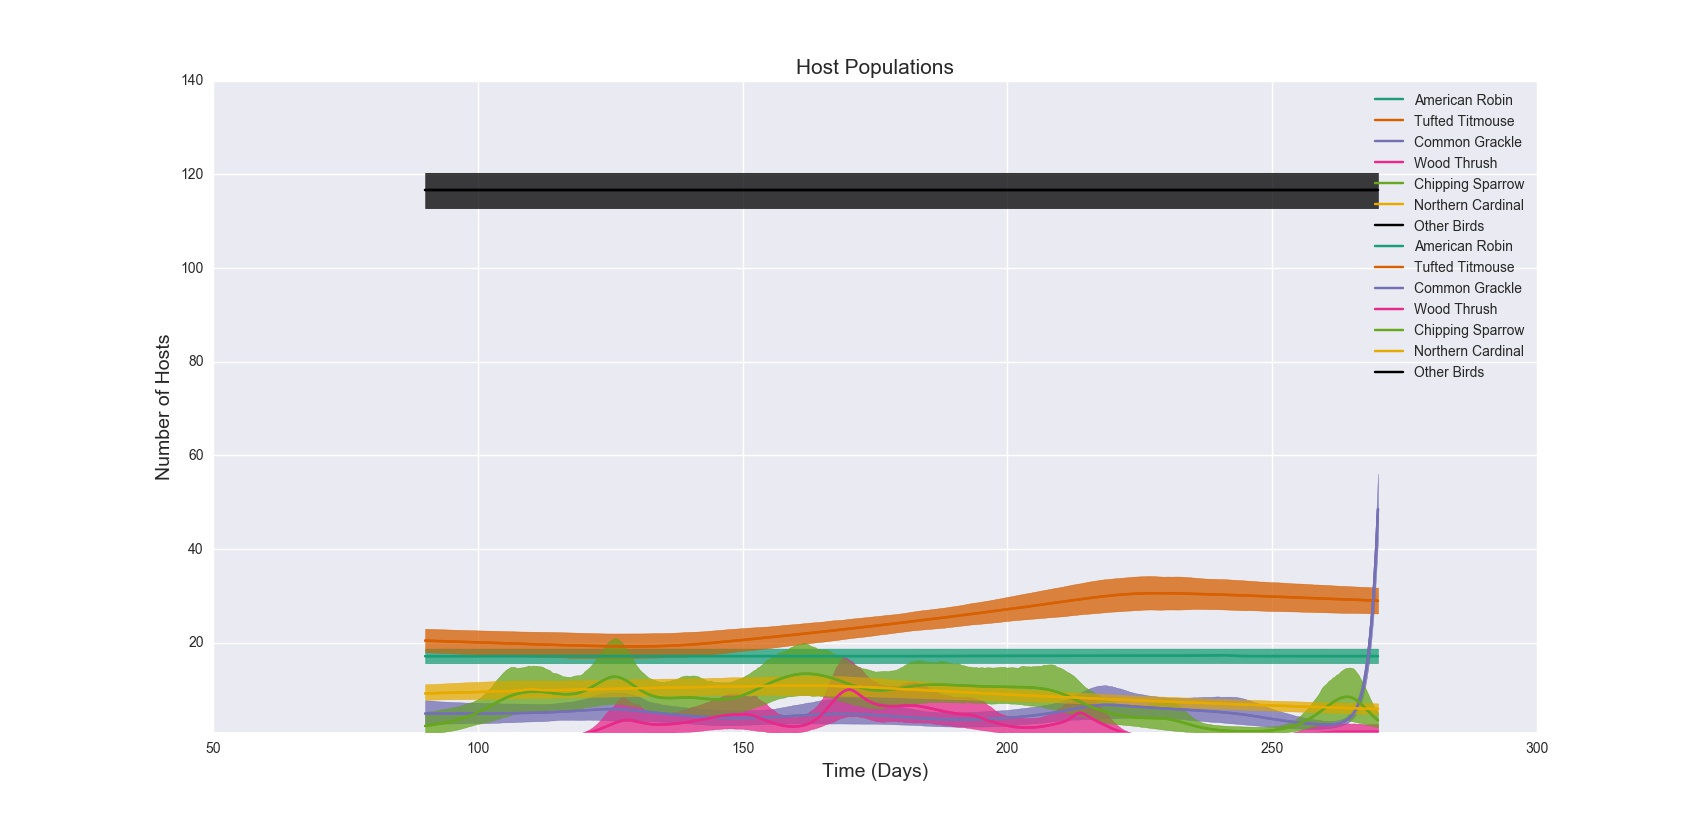
\includegraphics[width=\linewidth]{Populations}
\end{center}


\section*{Observed Feeding Preference}
Utilizing the population splines and calculated feeding indicies, we are able to see the observed feeding preference of the vector. \\
\begin{center}
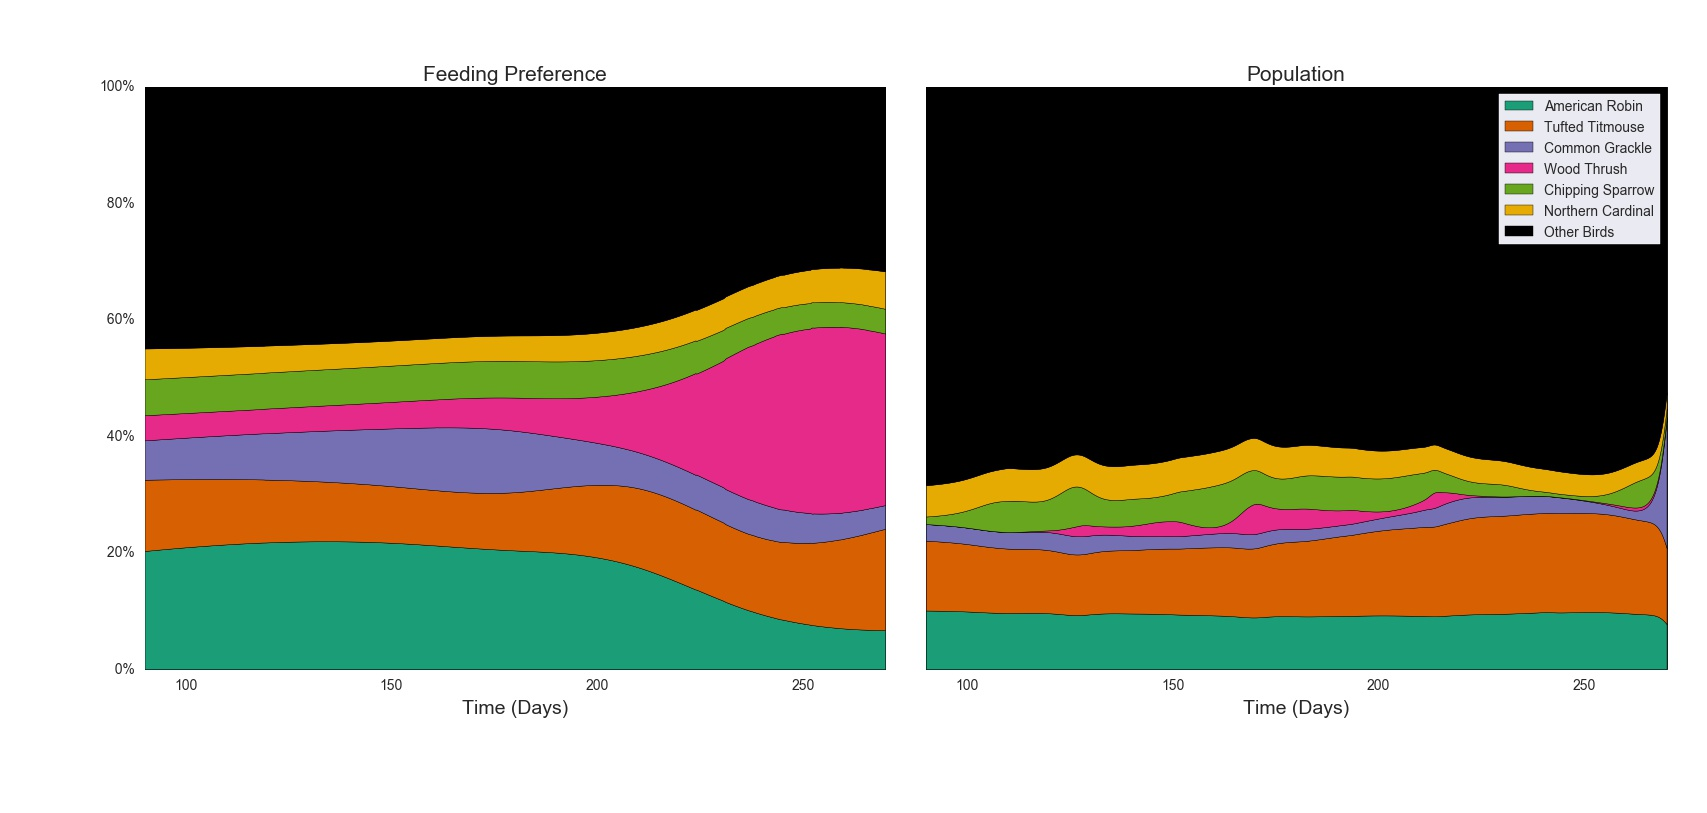
\includegraphics[width=\linewidth]{FeedingPreference}
\end{center}
 
\columnbreak

 \section*{Mathematical Model}
We choose to focus on 6 preferential host species, and a seventh consisting of all other birds.  This leaves us with a system of 23 differential equations (with i=1,2,...,9). \\
\begin{align*}
\frac{dS_i}{dt} &= \textit{b}N_i - \lambda_bS_i - \textit{d}S_i&  
\lambda_b &= \frac{\beta_1vI_v\sum\alpha_i}{\sum\alpha_iN_i} \\
\frac{dI_i}{dt} &=  \lambda_bS_i -  \gamma_bI_i-d_{EEE}I_i - \textit{d}I_i \\
\frac{dR_i}{dt} &= \gamma_bI_i - \textit{d}R_i&
\lambda_v &= \frac{\beta_2v\sum\alpha_II_i}{\sum\alpha_iN_i} \\
\frac{dI_v}{dt} &= \lambda_vS_v - d_vI_v \\
\frac{dS_v}{dt} &= r(t)N_v - d_vI_v&
\end{align*}

\section*{Results}
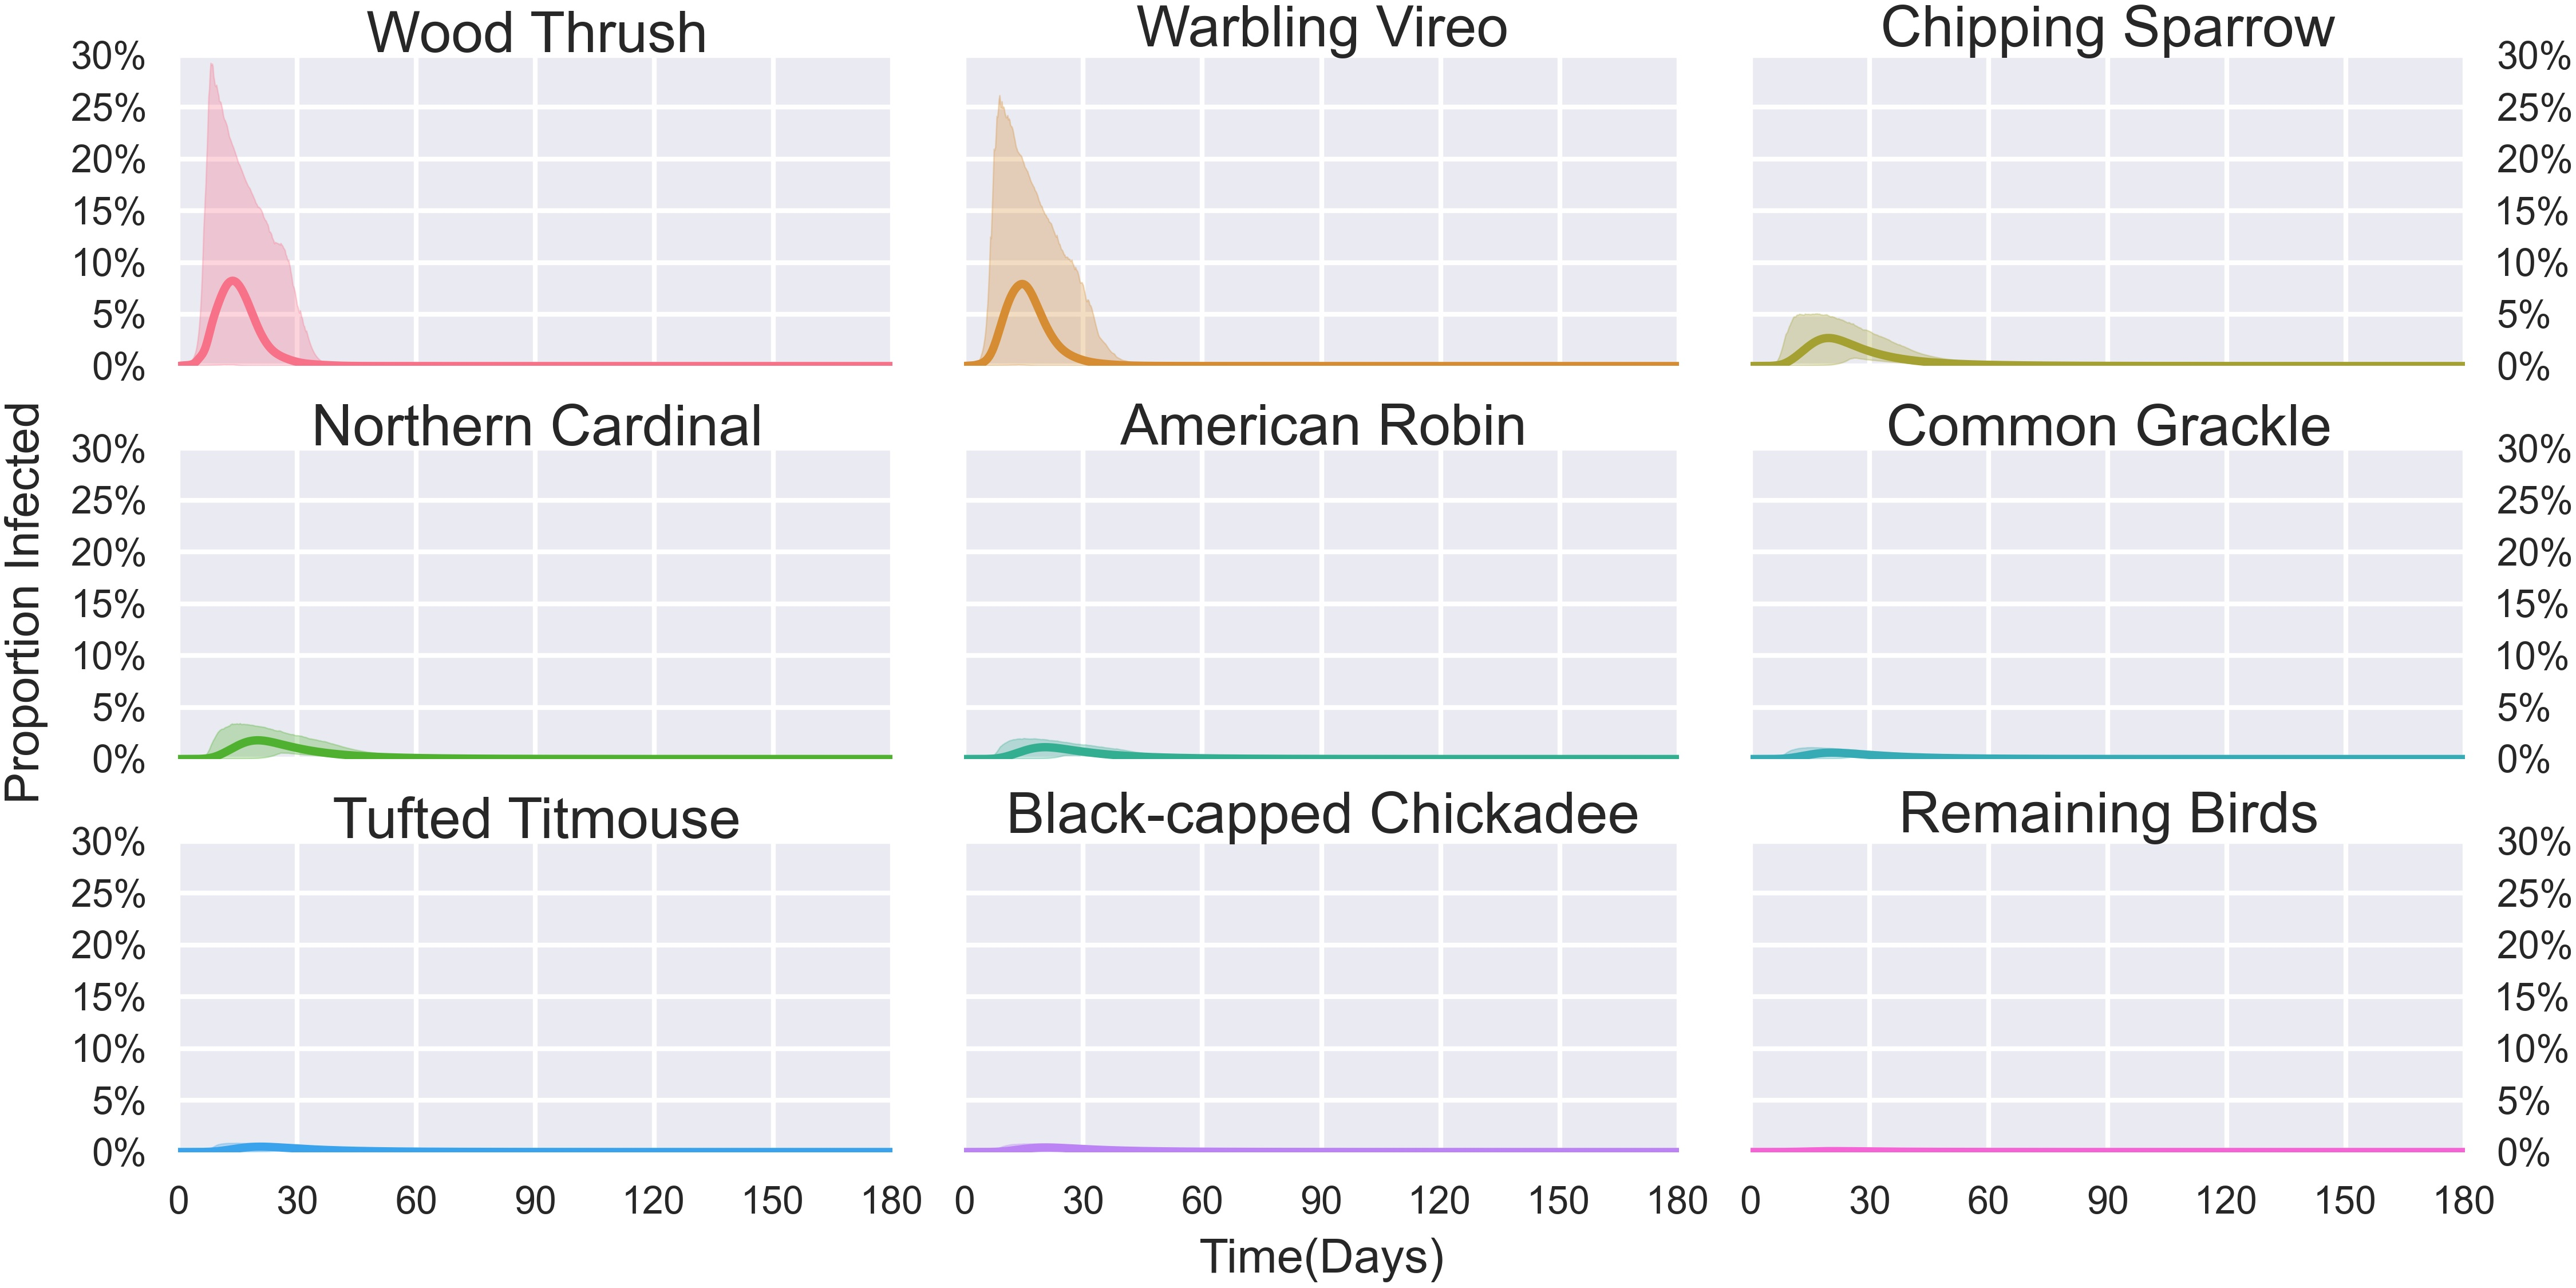
\includegraphics[width=\linewidth]{Results}

\section*{Conclusions}
Early in the season, the disease persists due to infections from preferntial species such as the Common Grackle and Amerian Robin.  Due to a increased feeding preference for Wood Thrush later in the season, in conjucture with the small overall population of Wood Thrush, lead to the population to quickly become infected.  This spike in new infections leads to an increase in in infections across all other species. 

\subsection*{Funding}
Funded in part by NIH U01 GM070694

\end{multicols}


\end{document}
